\documentclass[twoside]{book}

% Packages required by doxygen
\usepackage{fixltx2e}
\usepackage{calc}
\usepackage{doxygen}
\usepackage[export]{adjustbox} % also loads graphicx
\usepackage{graphicx}
\usepackage[utf8]{inputenc}
\usepackage{makeidx}
\usepackage{multicol}
\usepackage{multirow}
\PassOptionsToPackage{warn}{textcomp}
\usepackage{textcomp}
\usepackage[nointegrals]{wasysym}
\usepackage[table]{xcolor}

% Font selection
\usepackage[T1]{fontenc}
\usepackage[scaled=.90]{helvet}
\usepackage{courier}
\usepackage{amssymb}
\usepackage{sectsty}
\renewcommand{\familydefault}{\sfdefault}
\allsectionsfont{%
  \fontseries{bc}\selectfont%
  \color{darkgray}%
}
\renewcommand{\DoxyLabelFont}{%
  \fontseries{bc}\selectfont%
  \color{darkgray}%
}
\newcommand{\+}{\discretionary{\mbox{\scriptsize$\hookleftarrow$}}{}{}}

% Page & text layout
\usepackage{geometry}
\geometry{%
  a4paper,%
  top=2.5cm,%
  bottom=2.5cm,%
  left=2.5cm,%
  right=2.5cm%
}
\tolerance=750
\hfuzz=15pt
\hbadness=750
\setlength{\emergencystretch}{15pt}
\setlength{\parindent}{0cm}
\setlength{\parskip}{3ex plus 2ex minus 2ex}
\makeatletter
\renewcommand{\paragraph}{%
  \@startsection{paragraph}{4}{0ex}{-1.0ex}{1.0ex}{%
    \normalfont\normalsize\bfseries\SS@parafont%
  }%
}
\renewcommand{\subparagraph}{%
  \@startsection{subparagraph}{5}{0ex}{-1.0ex}{1.0ex}{%
    \normalfont\normalsize\bfseries\SS@subparafont%
  }%
}
\makeatother

% Headers & footers
\usepackage{fancyhdr}
\pagestyle{fancyplain}
\fancyhead[LE]{\fancyplain{}{\bfseries\thepage}}
\fancyhead[CE]{\fancyplain{}{}}
\fancyhead[RE]{\fancyplain{}{\bfseries\leftmark}}
\fancyhead[LO]{\fancyplain{}{\bfseries\rightmark}}
\fancyhead[CO]{\fancyplain{}{}}
\fancyhead[RO]{\fancyplain{}{\bfseries\thepage}}
\fancyfoot[LE]{\fancyplain{}{}}
\fancyfoot[CE]{\fancyplain{}{}}
\fancyfoot[RE]{\fancyplain{}{\bfseries\scriptsize Generated by Doxygen }}
\fancyfoot[LO]{\fancyplain{}{\bfseries\scriptsize Generated by Doxygen }}
\fancyfoot[CO]{\fancyplain{}{}}
\fancyfoot[RO]{\fancyplain{}{}}
\renewcommand{\footrulewidth}{0.4pt}
\renewcommand{\chaptermark}[1]{%
  \markboth{#1}{}%
}
\renewcommand{\sectionmark}[1]{%
  \markright{\thesection\ #1}%
}

% Indices & bibliography
\usepackage{natbib}
\usepackage[titles]{tocloft}
\setcounter{tocdepth}{3}
\setcounter{secnumdepth}{5}
\makeindex

% Hyperlinks (required, but should be loaded last)
\usepackage{ifpdf}
\ifpdf
  \usepackage[pdftex,pagebackref=true]{hyperref}
\else
  \usepackage[ps2pdf,pagebackref=true]{hyperref}
\fi
\hypersetup{%
  colorlinks=true,%
  linkcolor=blue,%
  citecolor=blue,%
  unicode%
}

% Custom commands
\newcommand{\clearemptydoublepage}{%
  \newpage{\pagestyle{empty}\cleardoublepage}%
}

\usepackage{caption}
\captionsetup{labelsep=space,justification=centering,font={bf},singlelinecheck=off,skip=4pt,position=top}

%===== C O N T E N T S =====

\begin{document}

% Titlepage & ToC
\hypersetup{pageanchor=false,
             bookmarksnumbered=true,
             pdfencoding=unicode
            }
\pagenumbering{roman}
\begin{titlepage}
\vspace*{7cm}
\begin{center}%
{\Large My Project }\\
\vspace*{1cm}
{\large Generated by Doxygen 1.8.11}\\
\end{center}
\end{titlepage}
\clearemptydoublepage
\tableofcontents
\clearemptydoublepage
\pagenumbering{arabic}
\hypersetup{pageanchor=true}

%--- Begin generated contents ---
\chapter{File Index}
\section{File List}
Here is a list of all files with brief descriptions\+:\begin{DoxyCompactList}
\item\contentsline{section}{\hyperlink{Lab1_8c}{Lab1.\+c} }{\pageref{Lab1_8c}}{}
\end{DoxyCompactList}

\chapter{File Documentation}
\hypertarget{RadixSort_8cpp}{}\section{Radix\+Sort.\+cpp File Reference}
\label{RadixSort_8cpp}\index{Radix\+Sort.\+cpp@{Radix\+Sort.\+cpp}}
{\ttfamily \#include $<$iostream$>$}\\*
Include dependency graph for Radix\+Sort.\+cpp\+:
\nopagebreak
\begin{figure}[H]
\begin{center}
\leavevmode
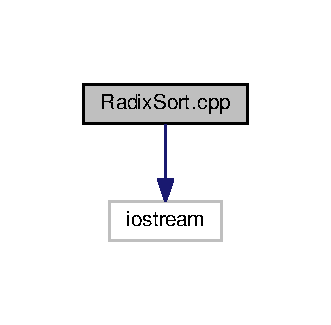
\includegraphics[width=159pt]{RadixSort_8cpp__incl}
\end{center}
\end{figure}
\subsection*{Functions}
\begin{DoxyCompactItemize}
\item 
int \hyperlink{RadixSort_8cpp_abcaeff5166458feccaf41175c9e6f757}{get\+Max} (int arr\mbox{[}$\,$\mbox{]}, int n)
\item 
void \hyperlink{RadixSort_8cpp_a6d0c3b80e7e567a24a09e50303770136}{count\+Sort} (int arr\mbox{[}$\,$\mbox{]}, int n, int exp)
\item 
void \hyperlink{RadixSort_8cpp_a6a9bec157182798edbf15f03dda6370a}{radixsort} (int arr\mbox{[}$\,$\mbox{]}, int n)
\item 
int \hyperlink{RadixSort_8cpp_ae66f6b31b5ad750f1fe042a706a4e3d4}{main} ()
\end{DoxyCompactItemize}


\subsection{Function Documentation}
\index{Radix\+Sort.\+cpp@{Radix\+Sort.\+cpp}!count\+Sort@{count\+Sort}}
\index{count\+Sort@{count\+Sort}!Radix\+Sort.\+cpp@{Radix\+Sort.\+cpp}}
\subsubsection[{\texorpdfstring{count\+Sort(int arr[], int n, int exp)}{countSort(int arr[], int n, int exp)}}]{\setlength{\rightskip}{0pt plus 5cm}void count\+Sort (
\begin{DoxyParamCaption}
\item[{int}]{arr\mbox{[}$\,$\mbox{]}, }
\item[{int}]{n, }
\item[{int}]{exp}
\end{DoxyParamCaption}
)}\hypertarget{RadixSort_8cpp_a6d0c3b80e7e567a24a09e50303770136}{}\label{RadixSort_8cpp_a6d0c3b80e7e567a24a09e50303770136}

\begin{DoxyCode}
17 \{
18     \textcolor{comment}{// Count[i] array will be counting the number of array values having that 'i' digit at their (exp)th
       place.  }
19     \textcolor{keywordtype}{int} output[n], i, count[10] = \{0\};
20  
21     \textcolor{comment}{// Count the number of times each digit occurred at (exp)th place in every input.}
22     \textcolor{keywordflow}{for} (i = 0; i < n; i++)
23         count[(arr[i] / exp) % 10]++;
24  
25     \textcolor{comment}{// Calculating their cumulative count.}
26     \textcolor{keywordflow}{for} (i = 1; i < 10; i++)
27         count[i] += count[i-1];
28  
29     \textcolor{comment}{// Inserting values according to the digit '(arr[i] / exp) % 10' fetched into count[(arr[i] / exp) %
       10].}
30     \textcolor{keywordflow}{for} (i = n - 1; i >= 0; i--)
31     \{
32         output[count[(arr[i] / exp) % 10] - 1] = arr[i];
33         count[(arr[i] / exp) % 10]--;
34     \}
35  
36     \textcolor{comment}{// Assigning the result to the arr pointer of main().}
37     \textcolor{keywordflow}{for} (i = 0; i < n; i++)
38         arr[i] = output[i];
39 \}
\end{DoxyCode}
\index{Radix\+Sort.\+cpp@{Radix\+Sort.\+cpp}!get\+Max@{get\+Max}}
\index{get\+Max@{get\+Max}!Radix\+Sort.\+cpp@{Radix\+Sort.\+cpp}}
\subsubsection[{\texorpdfstring{get\+Max(int arr[], int n)}{getMax(int arr[], int n)}}]{\setlength{\rightskip}{0pt plus 5cm}int get\+Max (
\begin{DoxyParamCaption}
\item[{int}]{arr\mbox{[}$\,$\mbox{]}, }
\item[{int}]{n}
\end{DoxyParamCaption}
)}\hypertarget{RadixSort_8cpp_abcaeff5166458feccaf41175c9e6f757}{}\label{RadixSort_8cpp_abcaeff5166458feccaf41175c9e6f757}

\begin{DoxyCode}
7 \{
8     \textcolor{keywordtype}{int} max = arr[0];
9     \textcolor{keywordflow}{for} (\textcolor{keywordtype}{int} i = 1; i < n; i++)
10         \textcolor{keywordflow}{if} (arr[i] > max)
11             max = arr[i];
12     \textcolor{keywordflow}{return} max;
13 \}
\end{DoxyCode}
\index{Radix\+Sort.\+cpp@{Radix\+Sort.\+cpp}!main@{main}}
\index{main@{main}!Radix\+Sort.\+cpp@{Radix\+Sort.\+cpp}}
\subsubsection[{\texorpdfstring{main()}{main()}}]{\setlength{\rightskip}{0pt plus 5cm}int main (
\begin{DoxyParamCaption}
{}
\end{DoxyParamCaption}
)}\hypertarget{RadixSort_8cpp_ae66f6b31b5ad750f1fe042a706a4e3d4}{}\label{RadixSort_8cpp_ae66f6b31b5ad750f1fe042a706a4e3d4}

\begin{DoxyCode}
53 \{
54     \textcolor{keywordtype}{int} n, i;
55     cout<<\textcolor{stringliteral}{"\(\backslash\)nEnter the number of data element to be sorted: "};
56     cin>>n;
57  
58     \textcolor{keywordtype}{int} arr[n];
59     \textcolor{keywordflow}{for}(i = 0; i < n; i++)
60     \{
61         cout<<\textcolor{stringliteral}{"Enter element "}<<i+1<<\textcolor{stringliteral}{": "};
62         cin>>arr[i];
63     \}
64  
65     \hyperlink{RadixSort_8cpp_a6a9bec157182798edbf15f03dda6370a}{radixsort}(arr, n);
66  
67     \textcolor{comment}{// Printing the sorted data.}
68     cout<<\textcolor{stringliteral}{"\(\backslash\)nSorted Data "};
69     \textcolor{keywordflow}{for} (i = 0; i < n; i++)
70         cout<<\textcolor{stringliteral}{"->"}<<arr[i];
71     \textcolor{keywordflow}{return} 0;
72 \}\end{DoxyCode}


Here is the call graph for this function\+:
\nopagebreak
\begin{figure}[H]
\begin{center}
\leavevmode
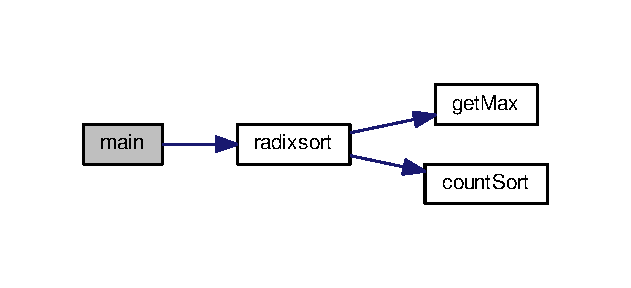
\includegraphics[width=303pt]{RadixSort_8cpp_ae66f6b31b5ad750f1fe042a706a4e3d4_cgraph}
\end{center}
\end{figure}


\index{Radix\+Sort.\+cpp@{Radix\+Sort.\+cpp}!radixsort@{radixsort}}
\index{radixsort@{radixsort}!Radix\+Sort.\+cpp@{Radix\+Sort.\+cpp}}
\subsubsection[{\texorpdfstring{radixsort(int arr[], int n)}{radixsort(int arr[], int n)}}]{\setlength{\rightskip}{0pt plus 5cm}void radixsort (
\begin{DoxyParamCaption}
\item[{int}]{arr\mbox{[}$\,$\mbox{]}, }
\item[{int}]{n}
\end{DoxyParamCaption}
)}\hypertarget{RadixSort_8cpp_a6a9bec157182798edbf15f03dda6370a}{}\label{RadixSort_8cpp_a6a9bec157182798edbf15f03dda6370a}

\begin{DoxyCode}
43 \{
44     \textcolor{keywordtype}{int} exp, m;
45     m = \hyperlink{RadixSort_8cpp_abcaeff5166458feccaf41175c9e6f757}{getMax}(arr, n);
46  
47     \textcolor{comment}{// Calling countSort() for digit at (exp)th place in every input.}
48     \textcolor{keywordflow}{for} (exp = 1; m/exp > 0; exp *= 10)
49         \hyperlink{RadixSort_8cpp_a6d0c3b80e7e567a24a09e50303770136}{countSort}(arr, n, exp);
50 \}
\end{DoxyCode}


Here is the call graph for this function\+:
\nopagebreak
\begin{figure}[H]
\begin{center}
\leavevmode
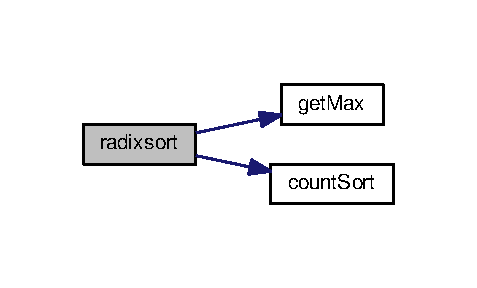
\includegraphics[width=229pt]{RadixSort_8cpp_a6a9bec157182798edbf15f03dda6370a_cgraph}
\end{center}
\end{figure}



%--- End generated contents ---

% Index
\backmatter
\newpage
\phantomsection
\clearemptydoublepage
\addcontentsline{toc}{chapter}{Index}
\printindex

\end{document}
